\documentclass[12pt,a4paper]{article}
\usepackage[utf8]{inputenc}
\usepackage[english]{babel}
\usepackage{amsmath}
\usepackage{amsfonts}
\usepackage{amssymb}
\usepackage{graphicx}
\graphicspath{ {./graphics/} }

\usepackage{fullpage}

\usepackage{float}

\usepackage{tikz}
\usetikzlibrary{arrows,automata, positioning,calc,shapes.geometric}

\begin{document}

\section{Physical Design}
To solve the sokoban problem a robot capable of performing simple tasks concerned with moving the can and itself around the game map are needed.
The behaviours the robot should be able to perform define how the robot should be formed in order to accomplish its task of solving the sokoban problem.
Therefore first the capabilities of the robot are considered and how this is reflected in the robot design.


\subsection{System Behaviours}
The robot was decided to be build upon being able to execute simple behaviours.
The execution of the behaviours would then be controlled from the \textit{Brain},
this is illustrated in figure \ref{fig:behaviourSystem}.

% brain/behaviour diagram
\begin{figure}[H]
\center
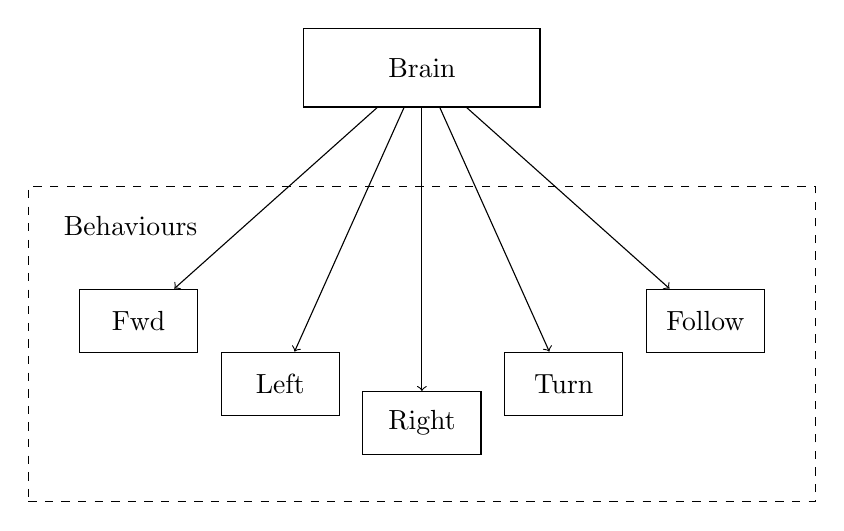
\begin{tikzpicture}[node distance=1cm]
%  behaviour box
\node[rectangle,draw,minimum width=10cm, minimum height=4cm, dashed, name=behaviour_box]  at (0,0) {};
\node[name=behaviour] at (-3.7,1.5) {Behaviours};

% Brain node 
\node[rectangle,draw,minimum width=3cm, minimum height=1cm, name=brain, above=of behaviour_box] {Brain};

% behaviours
\node[rectangle,draw,minimum width=1.5cm, minimum height=0.8cm, name=fwd] at (-3.6,0.3) {Fwd};
\node[rectangle,draw,minimum width=1.5cm, minimum height=0.8cm, name=left] at (-1.8,-0.5) {Left};
\node[rectangle,draw,minimum width=1.5cm, minimum height=0.8cm, name=right] at (0,-1.) {Right};
\node[rectangle,draw,minimum width=1.5cm, minimum height=0.8cm, name=turn] at (1.8,-0.5) {Turn};
\node[rectangle,draw,minimum width=1.5cm, minimum height=0.8cm, name=follow] at (3.6,0.3) {Follow};

% arrows inside 
\draw[->] (brain) -- (fwd) ;
\draw[->] (brain) -- (left) ;
\draw[->] (brain) -- (right) ;
\draw[->] (brain) -- (follow) ;
\draw[->] (brain) -- (turn) ;
\end{tikzpicture}
\caption{Overview of the systems behaviours.}
\label{fig:behaviourSystem}
\end{figure}

Here the central unit, the \textit{Brain} is responsible for finding the solution to the sokoban problem by invoking the five behaviours.
The \textit{Brain} is hence a combination of both the computer processing the map offline and the Lego-robot online when using the offline generated data to solve the puzzle.

The behaviours are defined in table \ref{tab:behaviourExplained} and based on dividing the behaviours into simple tasks which are easy to program.

\begin{table}[H]
\center
\begin{tabular}{c|l}
Behaviour & Description \\ \hline
Fwd & Makes the robot go straight ahead in the next intersection. \\
Left / Right & The robot turns left/right in the next intersection. \\
Turn & Turns the robot 180 degrees around in the next intersection. \\
Follow & Makes the robot follow the line till next intersection.
\end{tabular}
\caption{Behaviour table.}
\label{tab:behaviourExplained}
\end{table}

With these five behaviours the robot should then be able to navigate around the map and when a tomato can is encountered, push it to its destination.

\subsection{Physical Structure}
The structure of the robot should allow the movement of the robot across the map. 
That means, the robot should have at least two motors to move in the plane of the circuit and a minimum of two light sensors to check its position referred to the black lines of the map and check when the robot has arrived to a crossroad.

The chosen motor configuration consist in the use of two motors that move two parallel wheels. 
This allows the robot to change the direction of the movement setting a different motor speed on each motor.

Two light sensors are used as seen in figure \ref{fig:robotscheme}. 
In the position control, the value of the sensors are compared and the robot is controlled having in mind that the value of the sensors should be the same when the robot is centred above the line.
When the value of both sensors are low, the robot is facing a crossroad.

The position of the light sensors is in the front of the robot, and the distance between them should be enough to correctly detect the line. 
This means the light sensors should be placed close to the edges of the line such that they both detect a part of the line.
This means that the distance between them should be around the width of the line itself as shown in figure \ref{fig:robotscheme}.

\begin{figure}[H]
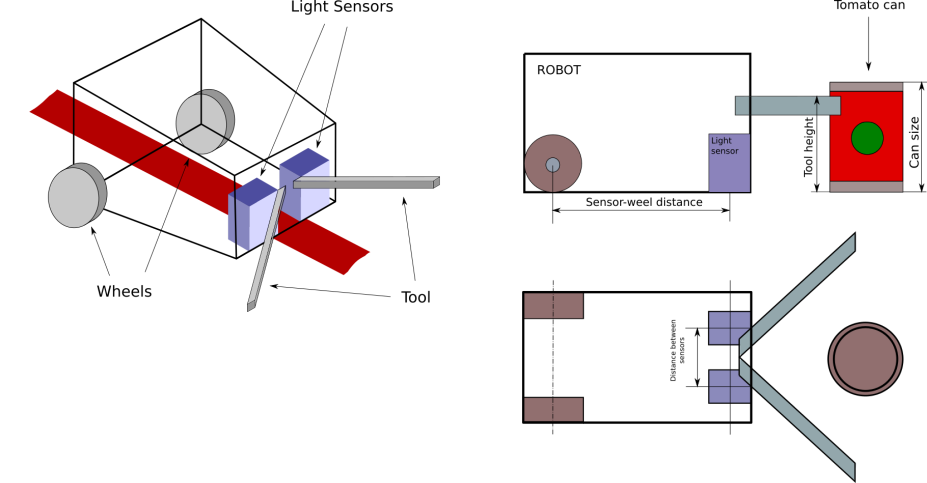
\includegraphics[width=10cm]{Fig2.png}
\centering
\caption{Scheme of the proposed configuration.}
\label{fig:robotscheme}
\end{figure}

To be able to push and guide the can across the map, the robot should have a proper tool that allows this task. 
The proposed design consist in two bars placed making an angle in a lower height than the one of the bottle. That allows the guide of the bottle when driving straight forward, as is shown in Figure 3. This configuration allows catching the can even when its position is displaced, making the robot's job more easy.

Thinking now about the behaviours of the robot, it can be assumed that when turning left or right and going fordward we wont move the can. Because of that, no special design requirements are needed. The turning back behaviour is more difficult. As the distance between lines is short, the turn back should be done in a small place because the sensors should find the line before the crossroad.

The position of the light sensors is in the front of the robot, and the distance between them should be enough to detect correctly the line. This means the light sensors should be placed close to the edges of the line, and because of that the distance between them should be around the width of the line.

Considering the rules of the game then the can is not permitted to be pushed left or right and because of that, no special design enabling this are required. 
The turning back behaviour is more difficult. 
%As the distance between the lines are short, the turn back should be done in a small place because the sensors should find the line before the crossroad.
The distance between the line intersections are short and the turn back has to happen in free space without interacting with the nearby placed cans.
On the same time, the robot should also finish the turn before reaching the new intersection.
Therefore the robot should not take up too much space, such that this can happen unproblematic and in a simple way.

The final build of the robot is seen in figure \ref{fig:robotImage}.

\begin{figure}[H]
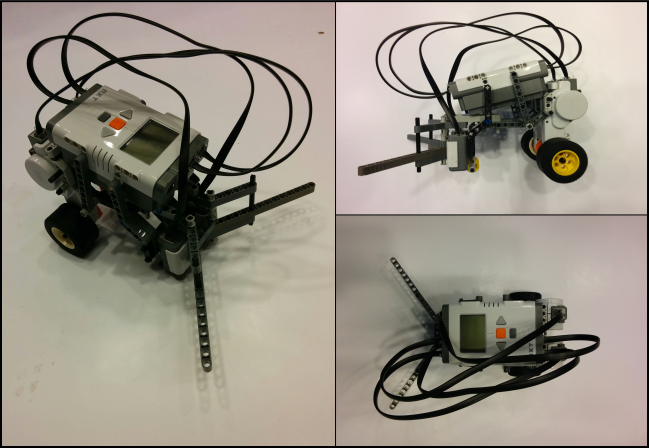
\includegraphics[width=10cm]{Fig1.png}
\centering
\caption{Images of the built robot.}
\label{fig:robotImage}
\end{figure}



% img of robot (schematic)

\end{document}